\documentclass[letterpaper,12pt]{article}

% Packages
%\usepackage{graphicx}
\usepackage{tikz,pgfplots}
\pgfplotsset{compat=1.15}
\usepackage{amsmath}
\usepackage[version=4]{mhchem}
\usepackage{siunitx}
\usepackage{esvect}


% Configuration
% Unit display preferences
\sisetup{per-mode = symbol-or-fraction,inter-unit-product = \ensuremath{{}\cdot{}}}
%\sisetup{per-mode = fraction,inter-unit-product = \ensuremath{{}\cdot{}}}

\begin{document}
\pagestyle{plain}
%\markright{Valuation}

\title{PHYS212 - Chap 21 Notes - Coulomb's Law}
\author{Sam Nelson}
\date{5/6/2020}
\maketitle

\section{Introduction}

\textit{Electrostatic force exerted by charged particles}

Charles-Augustin de Coulomb - 1785

The mathmatical form of the law (vector):

\begin{equation} \label{x1}
	\vec{F} = k\frac{q_1 q_2}{r^2}\hat{r}
\end{equation}

Where:

\begin{tabular}{l|l}
	$q_1$ & Charge 1 \\
	$q_2$ & Charge 2 \\
	$r$ & Particle separation \\
	$\hat{r}$ & Unit vector \\
	$k$ & Electrostatic/Coulomb Constant \\
\end{tabular}

Note the similarity between Coulomb's law and Newton's equation for the gravitational force between two particles

\begin{equation}
	\vv*{F} = G\frac{m_1 m_2}{r^2}\hat{r}
\end{equation}

The unit of charge is known as a \textit{Coulomb} and is defined in relation to the 
\textit{Ampere}

\begin{equation} \label{x2}
	i = \frac{dq}{dt}
\end{equation}

In this case, current is defined as the rate at which charge moves past a point or region.

Re-arranging, the units are related as so:

\begin{equation}
	1C = 1A \times 1s
\end{equation}

The magnitude of the electrostatic force is represented by:

\begin{equation}
	F = \frac{1}{4\pi\epsilon_0}\frac{|q_1||q_2|}{r^2}
\end{equation}


where $k = \frac{1}{4\pi\epsilon_0} = \SI{8.99e9}{\newton\meter\squared\per\coulomb\squared}$

or

\begin{equation}
	k = \frac{1}{4\pi\epsilon_0} = \SI{8.99e9}{\newton\meter\squared\per\coulomb\squared}
\end{equation}

with $\epsilon_0$ known as the \textit{Permittivity constant}
\begin{equation}
	\epsilon_0 = \SI{8.85e-12}{\coulomb\squared\per\newton\meter\squared}
\end{equation}

Principle of superposition. To find the net force on a particle, sum all the forces acting on that
particle.

\begin{equation}
	\vec{F_{1,net}} = \vec{F_{12}} + \vec{F_{13}} + \vec{F_{14}} + \vec{F_{15}} + \cdots + \vec{F_{1n,}}
\end{equation}

\begin{equation}
	\vv*{F}{1,\text{net}} = \vv*{F}{12} + \vv*{F}{13} + \vv*{F}{14} + \vv*{F}{15} + \cdots + \vv*{F}{1n,}
\end{equation}

%\begin{figure}[h]
%	\centering
%	\includegraphics[scale=0.8]{sine}
%	\caption{$\sin(x)$}
%	\label{sine}
%\end{figure}

%\begin{tikzpicture}
%	\begin{axis}[domain=3/4:5/4,legend pos=outer north east,trig format plots=rad]
%		\addplot {sin(2*pi*x)}; 
%		\addplot {cos(2*pi*x)}; 
%		\legend{$\sin(2 \pi x)$,$\cos(2 \pi x)$}
%	\end{axis}
%\end{tikzpicture}

\paragraph{Shell theory 1} A charged particle outside a shell with charge uniformly distributed on its surface is attracted to or repelled as if the shell's charge were concentrated as a particle at its center.

\paragraph{Shell theory 2} A charged particle inside a shell with charge uniformly disributed on its surface has no net force acting on it due to the shell.

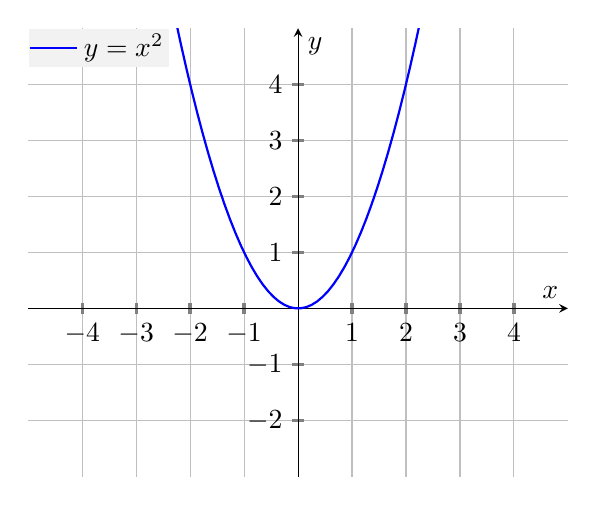
\begin{tikzpicture}
\begin{axis}[
  axis lines=middle,
  grid=major,
  xmin=-5,
  xmax=5,
  ymin=-3,
  ymax=5,
  xlabel=$x$,
  ylabel=$y$,
  xtick={-4,-3,...,4},
  ytick={-2,-1,...,4},
  tick style={very thick},
  legend style={
  at={(rel axis cs:0,1)},
  anchor=north west,draw=none,inner sep=0pt,fill=gray!10}
]
\addplot[blue,thick,samples=100] {x^2};
\addlegendentry{$y=x^2$}
\end{axis}
\end{tikzpicture}

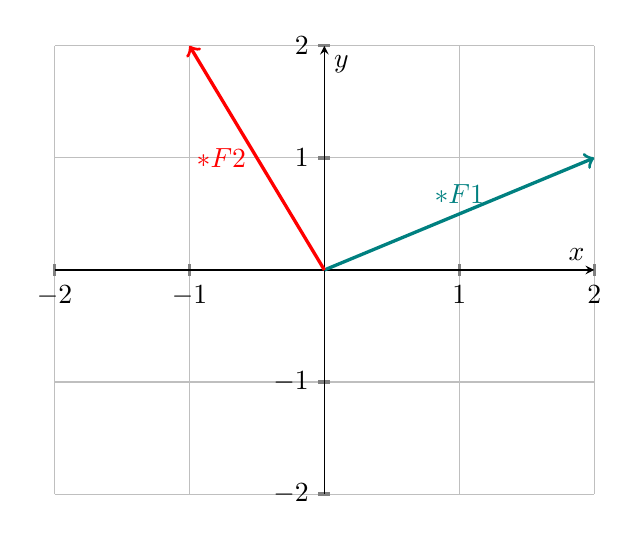
\begin{tikzpicture}
\begin{axis}[
  axis lines=middle,
  grid=major,
  xmin=-2,
  xmax=2,
  ymin=-2,
  ymax=2,
  xlabel=$x$,
  ylabel=$y$,
  xtick={-2,-1,...,2},
  ytick={-2,-1,...,2},
  tick style={very thick},
]
\draw [->,very thick,teal] (0,0) -- node[above] {$\vv*{F}{1}$} (2,1);
	\draw [->,very thick,red] (0,0) -- node[below,left] {$\vv*{F}{2}$} (-1,2);
\end{axis}
\end{tikzpicture}

\section{Quantization of Charge}

Any positive or negative charge $q$ that can be detected, can be written as

\begin{equation}
	q = ne, \quad n = \pm 1, \pm 2, \pm 3, \dots ,
\end{equation}

In which $e$, the \textbf{elementary charge,} has the approximate value

\begin{equation}
	e = \SI{1.602e-19}{\coulomb}
\end{equation}

\section{Conservation of Charge}

Charge is not created or destroyed, it is transfered. This hypothesis is known as \textbf{conservation of charge}.

An example is the radioactive decay of uranium-238 ($\ce{^{238}_{}U}$).

\begin{equation}
	\ce{^{238}_{}U -> ^{234}_{}Th + ^{4}_{}He,}
\end{equation}

The \textit{parent} nucleus $\ce{^{238}_{}U}$ contains 92 protons, with a charge of $+92e$, the \textit{daughter} nucleus \ce{^{234}_{}Th} contains 90 protons, with a charge of $+90e$ and the emitted alpha particle \ce{^{4}_{}He} contains 2 protons, with a charge of $+2e$. Total charge is $+92e$ before and after the decay, thus charge is conserved.

Another example of this charge conservation is when an electron $\mathrm{e}^-$ (charge $-e$) and its antiparticle, the \textit{positron} $\mathrm{e}^+$ (charge $+e$), undergo an \textit{annihilation process}, transforming into two \textit{gamma rays}:

\begin{equation}
	e^- + e^+ \longrightarrow \gamma + \gamma \quad \text{(annihilation).}
\end{equation}

\end{document}
